\let\xn\xnote
\section{Results}

\subsection{Metrics}

\begin{figure}[htbp]
    \centering
    \includesvg[width=\textwidth,height=\textheight,keepaspectratio]{Sections/Figures/judges_normalised_svg.svg}
    \caption{Citation count by Justice of the High Court of Australia.}
\end{figure}

\subsection{Causes}

%TC:ignore
% \begin{longtable}{lllll}
%     \caption{GLMM coefficients and corresponding statistical significance.}
%     \endfirsthead
%     \toprule
%     \endhead
%     \bottomrule
%     \multicolumn{4}{l}{\PStar{\emph{p} < 0.05} \ \ \PStar{\PStar{\emph{p} < 0.01}} \ \ \PStar{\PStar{\PStar{\emph{p} < 0.001}}}}
%     \endlastfoot
%     \toprule
%     {} & {\textbf{Model 1}}     & {\textbf{Model 2}}            & {\textbf{Model 3}}            & {\textbf{Model 4}}                                      \\ \midrule
%     \textbf{Judgment Length}    & \Star{\Star{\Star{0.004}}}    & \Star{\Star{\Star{0.004}}}    & \Star{\Star{0.002}}        & \Star{\Star{\Star{0.001}}} \\
%     \textbf{Coram Size}         &                               & 0.143                         & 0.175                      & 0.178                      \\
%     \textbf{Lone Opinion}       &                               &                               & \Star{\Star{\Star{1.553}}} & \Star{\Star{\Star{1.770}}} \\
%     \textbf{ALP Appointee}      &                               &                               &                            & \Star{\Star{1.971}}        \\ \midrule
%     \textbf{Log Likelihood}     & -1584.287                     & -1570.858                     & -1278.506                  & -1298.995                  \\
%     \textbf{AIC} & 3178.574     &  3159.717                     &  2585.012                     & 2627.991                                                \\
% \end{longtable}
%TC:endignore

\begin{longtable}{lrrrrrr}
    \caption{GLMM coefficients for citations to journal articles by the High Court.}
    \endfirsthead
    \toprule
    \endhead
    \bottomrule
    \multicolumn{6}{l}{\PStar{\emph{p}} < 0.001. Standard Error in parentheses.}
    \endlastfoot
    \toprule
    {}                          & {\textbf{Model 1}}            & {\textbf{Model 2}}            & {\textbf{Model 3}}            & {\textbf{Model 4}}           \\ \midrule
    \textbf{Judgment Length}    & \Star{0.003}                  & \Star{0.002}                  & \Star{0.003}                  & \Star{0.002}                 \\
                                & (0.000)                       & (0.000)                       & (0.000)                       & (0.000)                      \\
    \textbf{Lone Opinion}       &                               & \Star{1.445}                  &                               & \Star{1.425}                 \\
                                &                               & (0.044)                       &                               & (0.044)                      \\
    \textbf{Coram Size}         &                               &                               & \Star{0.164}                  & \Star{0.129}                 \\
                                &                               &                               & (0.018)                       & (0.018)                      \\
    \textbf{Appeal Allowed}     &                               &                               & {-0.018\hphantom{0}}          &                              \\
                                &                               &                               & (0.033)                       &                              \\
    \textbf{Intercept}          & \Star{-1.153}                 & \Star{-1.264}                 & \Star{-2.020}                 & \Star{-1.951}                \\ 
                                & (0.130)                       & (0.097)                       & (0.171)                       & (0.143)                      \\ \midrule
    \textbf{Log Likelihood}     & -6907.74                     & -6388.22                     & -6861.92                     & -6361.75                        \\
    \textbf{AIC}                & 13823.48                     & 12786.45                     & 13735.84                     & 12735.50                        \\
\end{longtable}


\subsection{Rankings}


\begin{longtable}{llll}
    \caption{Authors cited on more than 20 occasions.}
    \endfirsthead
    \toprule
    \endhead
    \bottomrule
    \multicolumn{4}{r}{\emph{Continues on next page}}
    \endfoot
    \bottomrule
    \multicolumn{4}{l}{\PStar{International author}; \  \PCross{Australian judge}; \ \PCCross{Admitted as an Australian barrister}.}
    \endlastfoot

    \toprule
    {\textbf{Rank}} & {\textbf{Name}} & {\textbf{Score}} & {\textbf{Area of Expertise}} \\ \midrule
    1  & {\Cross{Anthony Mason}}            & 102 & {Public \& Private Law} \\
    2  & {\CCross{George Williams}}         &  71 & {Constitutional Law}  \\
    3  & {\Cross{Owen Dixon}}               &  69 & {Public \& Private Law} \\
    4  & {\Star{Glanville Williams}}         &  50 & {Criminal Law} \\
    5  & {\CCross{Enid Campbell}}           &  42 & {Constitutional \& Administrative Law}  \\ \midrule
    6  & {Anthony Gray}                      &  41 & {Public Law} \\
    7  & {Ian G. Campbell}                   &  40 & {Criminal Law} \\
    8  & {\Star{Frederic W. Maitland}}       &  36 & {Legal History}  \\
    9  & {\Star{Peter Birks}}                &  35 & {Equity} \\
    10 & {Cheryl Saunders}                   &  34 & {Public Law}  \\ \midrule
    11 & {\Star{Wesley N. Hohfeld}}          &  33 & {Jurisprudence} \\
    12 & {\Cross{Bruce H. McPherson}}       &  33 & {Equity \& Commercial Law} \\
    13 & {Geoffrey Sawer}                    &  32 & {Public \& Private Law} \\
    14 & {Belinda Smith}                     &  31 & {Anti-discrimination Law} \\
    15 & {\Star{Andrew Simester}}            &  30 & {Criminal Law}  \\ \midrule
    16 & {\Star{Theodore Waldman}}           &  28 & {Legal Theory} \\ 
    17 & {\Cross{Paul Brereton}}            &  27 & {Private \& International Law} \\
    18 & {\Cross{Stephen Gageler}}          &  27 & {Public \& Private Law} \\
    19 & {\Star{William S. Holdsworth}}      &  27 & {Legal History} \\
    20 & {\Star{A. W. Brian Simpson}}        &  26 & {Legal Historian \& Philosopher} \\ \midrule
    21 & {\Cross{Murray Gleeson}}           &  26 & {Public \& Private Law} \\ 
    22 & {Mark Aronson}                      &  26 & {Administrative Law} \\
    23 & {\Star{Paul A. Freund}}             &  25 & {Constitutional Law} \\
    24 & {\Cross{Michael Kirby}}            &  25 & {Public \& Private Law} \\
    25 & {William J. Ford}                   &  25 & {Tort and Industrial Relations Law} \\ \midrule
    26 & {\CCross{Jeremy Kirk}}             &  25 & {Public \& Private Law} \\ 
    27 & {Clifford L. Pannam}                &  24 & {Public \& Private Law} \\
    28 & {\Star{Roscoe Pound}}               &  23 & {Legal Theory} \\
    29 & {John W. Carter}                    &  21 & {Contract Law}  \\
    30 & {\CCross{Jane Stapleton}}          &  20 & {Tort Law} \\ \midrule
    31 & {D. M. Gordon}                      &  20 & {Public \& Private Law} \\ 
    32 & {\Cross{Paul Finn}}                &  20 & {Public \& Private Law} \\
\end{longtable}


%TC:ignore

% \begin{longtable}{cccc}
%     \caption{Authors ranked by influence}
%     \endfirsthead
%     \toprule
%     \endhead
%     \bottomrule
%     \multicolumn{4}{r}{\emph{Continues on next page}}
%     \endfoot
%     \bottomrule
%     \multicolumn{4}{l}{\textsuperscript{*} \ Denotes an international author.}
%     \endlastfoot

%     \toprule
%     {\textbf{Rank}} & {\textbf{Name}} & {\textbf{Score} ($10^{-3}$)} & {\textbf{Area of Expertise}} \\ \midrule
%     1  & {Leslie Zines}                     & 4.220 & {Constitutional Law} \\
%     2  & {Michael Pryles}                   & 3.930 & {Arbitration}  \\
%     3  & {Robert J. Sadler}                 & 1.980 & {Commercial Law} \\
%     4  & {\Star{Robert Jennings}}           & 1.690 & {International Law}  \\
%     5  & {Alex C. Castles}                  & 1.510 & {Legal History} \\ \midrule
%     6  & {Colin S. Phegan}                  & 1.450 & {Tort Law} \\
%     7  & {Victor Windeyer}                  & 1.370 & {Equity \& Commercial Law} \\ 
%     8  & {Adrienne Stone}                   & 1.350 & {Constitutional Law}  \\
%     9  & {Neil Morgan}                      & 1.320 & {Criminal Law} \\
%     10 & {George Williams}                  & 1.270 & {Constitutional Law}  \\ \midrule
%     11 & {Geoffrey Lindell}                 & 1.220 & {Constitutional Law} \\
%     12 & {Roger Douglas}                    & 1.220 & {Administrative Law} \\
%     13 & {Enid Campbell}                    & 1.200 & {Constitutional \& Administrative Law} \\
%     14 & {David McLauchlan}                 & 1.150 & {Contract \& Commercial Law} \\
%     15 & {Bernard Murphy}                   & 1.150 & {Class Actions} \\ \midrule
%     16 & {Camille Cameron}                  & 1.150 & {Civil Procedure} \\
%     17 & {\Star{Rachael Mulheron}}          & 1.150 & {Tort Law} \\
%     18 & {Allan Murray-Jones}               & 1.140 & {\textbf{TODO: research}} \\
%     19 & {Deborah DeMott}                   & 1.140 & {Equity \& Commercial Law} \\
%     20 & {Clarrie Harders}                  & 1.130 & {Constitutional Law} \\ \midrule
%     21 & {Bruce H. McPherson}               & 1.110 & {Equity \& Commercial Law} \\
%     22 & {Douglas Pike}                     & 1.090 & {Legal History} \\
%     23 & {Jeffrey Goldsworthy}              & 1.080 & {Constitutional Law} \\
%     24 & {Ronald Sackville}                 & 1.040 & {\textbf{TODO: research}} \\
%     25 & {Roland Keller}                    & 1.030 & {Criminal Law} \\ \midrule
%     26 & {Lance Wright}                     & 1.020 & {Industrial Relations Law} \\
%     27 & {Murray Gleeson}                   & 0.994 & {Public \& Private Law} \\
%     28 & {Anthony Mason}                    & 0.986 & {Public \& Private Law}  \\
%     29 & {John H. C. Morris}                & 0.975 & {Conflict of Laws} \\
%     30 & {Mark Aronson}                     & 0.935 & {Administrative Law} \\ \midrule
%     31 & {Nicola McGarrity}                 & 0.929 & {Public \& Criminal Law} \\
%     32 & {Dan Meagher}                      & 0.925 & {Constitutional Law} \\
%     33 & {Stephen Gageler}                  & 0.922 & {Public \& Private Law} \\
%     34 & {I. G. Campbell}                     & 0.922 & {Criminal Law} \\ 
%     35 & {\Star{Kent Roach}}                & 0.917 & {Criminal Law} \\ \midrule
%     36 & {Ben Golder}                       & 0.914      & {Legal Theory} \\
%     37 & {Anthony Reilly}                   & 0.914      & {\textbf{TODO}} \\
%     38 & {\Star{A. W. Brian Simpson}}       & 0.903      & {Legal Historian \& Philosopher} \\
%     39 & {Robin Creyke}                     & 0.899      & {Administrative Law} \\
%     40 & {\Star{Roderick Bagshaw}}          & 0.898      & {Administrative \& Tort Law} \\ \midrule
%     41 & {J. A. Andrews}                      & 0.885      & {\textbf{TODO}} \\
%     42 & {\Star{Glanville Williams}}        & 0.881      & {Criminal Law} \\
%     43 & {Neil Foster}                      & 0.878      & {Tort Law} \\
%     44 & {\Star{Brandon L. Garrett}}         & 0.876      & {Evidence} \\
%     45 & {Gary Edmond}                      & 0.876      & {Expert Evidence} \\ \midrule
%     46 & {\Star{Walder G. W. White}}        & 0.875      & {Family Law} \\
%     47 & {\Star{William Anson}}             & 0.874      & {Contract Law \& Equity} \\
%     48 & {Belinda Smith}                    & 0.873      & {Anti-discrimination Law} \\
%     49 & {Michael Kirby}                    & 0.868      & {Public \& Private Law} \\ 
%     50 & {\Star{Harry Kalven Jr}}           & 0.861      & {Tort Law} \\
% \end{longtable}

% % 

%TC:endignore

\begin{longtable}{llll}
    \caption{Authors ranked by influence (Min-Max normalised).}
    \endfirsthead
    \toprule
    \endhead
    \bottomrule
    \multicolumn{4}{r}{\emph{Continues on next page}}
    \endfoot
    \bottomrule
    \multicolumn{4}{l}{\textsuperscript{*} \ Denotes an international author.}
    \endlastfoot

    \toprule
    {\textbf{Rank}} & {\textbf{Name}} & {\textbf{Score}} & {\textbf{Area of Expertise}} \\ \midrule
    1  & {Leslie Zines}                     & 1.00000 & {Constitutional Law} \\
    2  & {Michael Pryles}                   & 0.89980 & {Arbitration}  \\
    3  & {Robert J. Sadler}                 & 0.35260 & {Commercial Law} \\
    4  & {\Star{Robert Jennings}}           & 0.27410 & {International Law}  \\
    5  & {Alex C. Castles}                  & 0.23260 & {Legal History} \\ \midrule
    6  & {Colin S. Phegan}                  & 0.21740 & {Tort Law} \\
    7  & {Victor Windeyer}                  & 0.19700 & {Equity \& Commercial Law} \\ 
    8  & {Adrienne Stone}                   & 0.19370 & {Constitutional Law}  \\
    9  & {Neil Morgan}                      & 0.18530 & {Criminal Law} \\
    10 & {George Williams}                  & 0.16550 & {Constitutional Law}  \\ \midrule
    11 & {Enid Campbell}                    & 0.15160 & {Constitutional \& Administrative Law} \\
    12 & {Geoffrey Lindell}                 & 0.15000 & {Constitutional Law} \\
    13 & {Anthony Mason}                    & 0.14730 & {Public \& Private Law} \\
    14 & {David McLauchlan}                 & 0.13920 & {Contract \& Commercial Law} \\
    15 & {Bruce H. McPherson}               & 0.13660 & {Equity \& Commercial Law} \\ \midrule
    16 & {Allan Murray-Jones}               & 0.13600 & {Constitutional Law} \\
    17 & {Bernard Murphy}                   & 0.13590 & {Class Actions} \\
    18 & {Camille Cameron}                  & 0.13590 & {Civil Procedure} \\
    19 & {\Star{Rachael Mulheron}}          & 0.13590 & {Tort Law} \\
    20 & {Deborah DeMott}                   & 0.13500 & {Equity \& Commercial Law} \\ \midrule
    21 & {Ronald Sackville}                 & 0.13150 & {Public \& Private Law} \\
    22 & {Clarrie Harders}                  & 0.13120 & {Constituional Law} \\
    23 & {Douglas Pike}                     & 0.12320 & {Legal History} \\
    24 & {Roland Keller}                    & 0.11960 & {Criminal Law} \\
    25 & {Jeffrey Goldsworthy}              & 0.11750 & {Constitutional Law} \\ \midrule
    26 & {Murray Gleeson}                   & 0.09910 & {Public \& Private Law} \\
    27 & {John H. C. Morris}                & 0.08887 & {Conflict of Laws} \\
    28 & {Stephen Gageler}                  & 0.08714 & {Public \& Private Law}  \\
    29 & {Roger Douglas}                    & 0.08246 & {Administrative Law} \\
    30 & {Dan Meagher}                      & 0.08119 & {Constitutional Law} \\ \midrule
    31 & {\Star{A. W. Brian Simpson}}       & 0.08083 & {Legal Historian \& Philosopher} \\
    32 & {Mark Aronson}                     & 0.07963 & {Administrative Law} \\
    33 & {Ian G. Campbell}                  & 0.07634 & {Criminal Law} \\
    34 & {Robin Creyke}                     & 0.07519 & {Administrative Law} \\ 
    35 & {\Star{Glanville Williams}}        & 0.07474 & {Criminal Law} \\ \midrule
    36 & {Belinda Smith}                    & 0.07352 & {Anti-discrimination Law} \\
    37 & {\Star{Roderick Bagshaw}}          & 0.07165 & {Administrative \& Tort Law} \\
    38 & {John A. Andrews}                  & 0.07091 & {Criminal Law} \\
    39 & {Lance Wright}                     & 0.06908 & {Industrial Relations Law} \\
    40 & {\Star{Brandon L. Garrett}}        & 0.06794 & {Evidence} \\ \midrule
    41 & {Gary Edmond}                      & 0.06794 & {Expert Evidence} \\
    42 & {\Star{Walder G. W. White}}        & 0.06756 & {Family Law} \\
    43 & {Neil Foster}                      & 0.06753 & {Tort Law} \\
    44 & {\Star{William Anson}}             & 0.06748 & {Public \& Private Law} \\
    45 & {\Star{Antonin Scalia}}            & 0.06547 & {Public \& Private Law} \\ \midrule
    46 & {\Star{Ian Loveland}}              & 0.06502 & {Public Law} \\
    47 & {\Star{Harry Kalven Jr}}           & 0.06415 & {Public \& Private Law} \\
    48 & {Owen Dixon}                       & 0.06358 & {Public \& Private Law} \\
    49 & {\Star{Stephen D. Sugarman}}       & 0.06310 & {Tort Law} \\ 
    50 & {Ernst Willheim}                   & 0.06286 & {Public Law} \\
\end{longtable}


% Sheehy and Dumay forcefully claim that the Sydney Law Review is the most cited journal by the High Court of Australia, however, this is not so.

% \begin{figure}[htbp]
%     \centering
%     \includesvg[width=\textwidth,height=\textheight,keepaspectratio]{Figures/journals_svg.svg}
%     \caption{Ranked list of top n journals cited by the High Court (n=30)}
% \end{figure}

% \begin{figure}[htbp]
%     \centering
%     \includesvg[width=\textwidth,height=\textheight,keepaspectratio]{Figures/authors_svg.svg}
%     \caption{Ranked list of top n authors cited by the High Court (n=30)}
% \end{figure}

% \begin{figure}
%   \centering
%   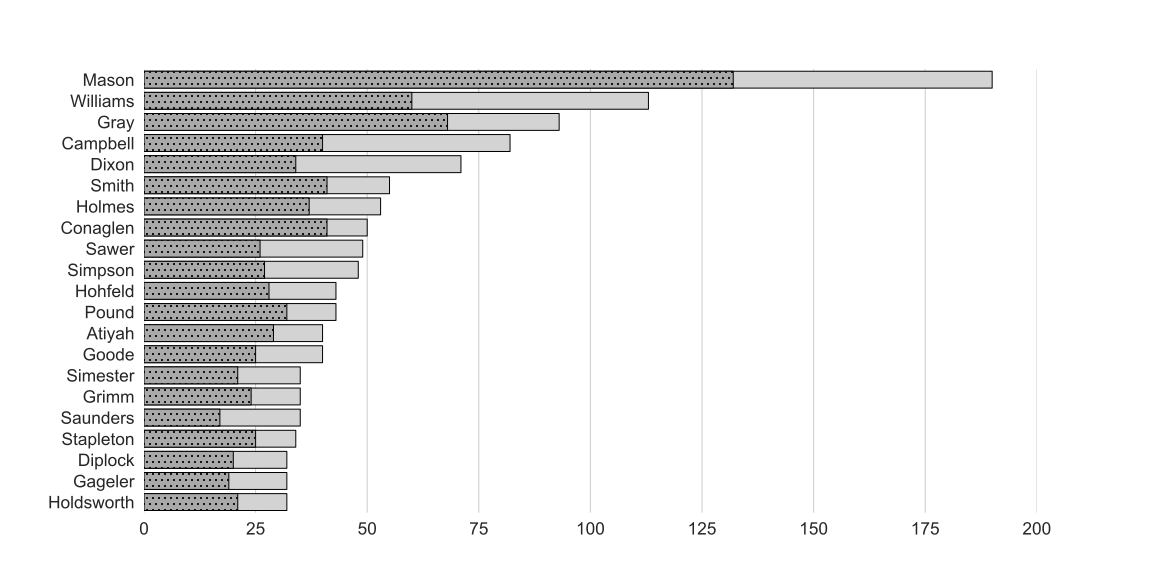
\includegraphics[]{Figs/authors.png}
%   \caption{fig.}
%   \label{fig:authors}
% \end{figure}
